\documentclass[paper=a4]{proc}
\usepackage[ngerman]{babel}

%Images
\usepackage{graphicx, svg}

%Tikz
\usepackage{tikz}
\usepackage{environ}
\usepackage{pgfplots}
\usepgfplotslibrary{fillbetween}
\usetikzlibrary{positioning}

\pagenumbering{gobble}		%Disable page numbers

\title{Graphical Data Visualization Tool}
\author{George Bellamy, Christoph Honal, Felix Wieser}

\begin{document}
	\maketitle
	\thispagestyle{plain}	%Disable page numbers
	\section{Outline}
		This project is about implementing a graphical user interface to interactively visualize the output of the SWE tsunami simulation and provide basic analysis functions. Additionally, the ability to export images, videos and graphs (i.e. cross-sections) is planned. This project is intended to be a standalone application that loads pre-calculated datasets.
	\section{Description}
		\subsection{GUI}
			The GUI consists mainly of a 2D renderer and some control elements. It  supports zoom/pan of the map and multiple layers of data to allow overlays.
			\subsubsection{General UI}
			Most of the screen space is dedicated to the rendered image.
			
			A toolbar is located above the image, that contains play and pause buttons, as well as a display for the current time. The playback speed can be adjusted in relation to real time via a set of speed control buttons, as well as a reset button to jump to the beginning of the simulation. Additionally, zoom control buttons allow to change the magnification of the rendered part of the map. The last button is a sticky selection pan button to move the current selection displayed in the renderer.
			
			On the top right next to the image is a data field to display data of a specific point from the simulation. Below this one can configure the renderer by selecting different data layers. Furthermore, one can choose the action on clicking (Which analysis method used) on the renderer (sticky selection). Finally, a list of the currently active sample points are located below.
			
			\begin{figure}
				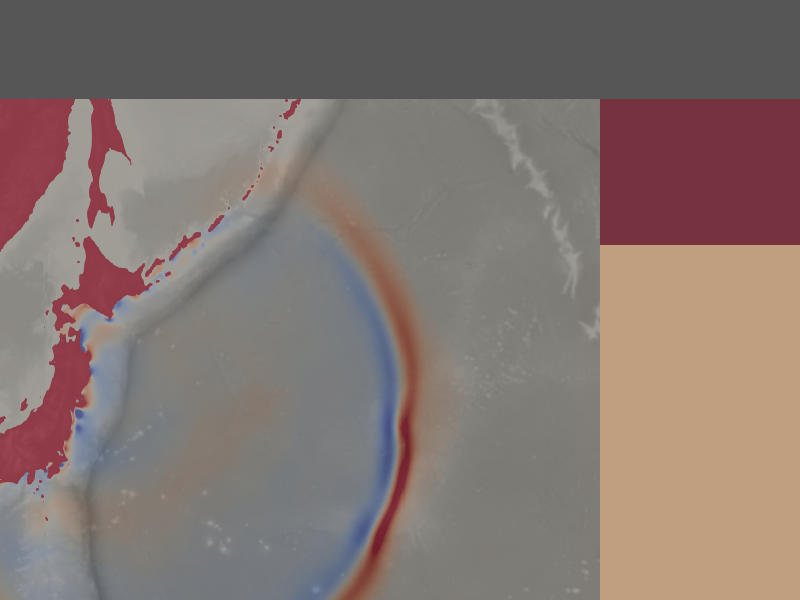
\includegraphics[clip, width=\linewidth]{../../presentation4/img/GUI.png}
				\caption*{\centering The basic layout of the GUI\newline Toolbar (gray), raw data field (red), list of sample points (brown)}
			\end{figure}
			
			\subsubsection{Data layers}
			\paragraph{Surface height only}\hspace{0pt}\newline
			This shows the bathymetry without water of the scenario before or after the earthquake so the effect of this can be seen. color gradients are used for height.
			
			\paragraph{Water and land height}\hspace{0pt}\newline
			Water and land is colored in different colors (Land green to gray, water blue to red) and displayed together, different color gradients indicate different height.
			
			\paragraph{Coastal damage estimation}\hspace{0pt}\newline
		 This probes all coastal regions and outputs the maximum wave height over time at each location as a color gradient on the land to water boarders. the exact value can be seen by mouseover in the data field 
		 %TODO this might be hard to implement, there may be an easier solutiuon
 		\subsection{Data analysis}
			The following analysis-tools are planned at this time:
			\subsubsection*{Cell probe}
				The user can select a point on the renderer (by mouseover) of which the values are shown in a data field next to the rendered image. It contains bathymetry and water height as well as coordinates. Once a position is clicked this becomes saved and over time values are shown such as maximum water height.
			\subsubsection*{Arrival time calculator}
				Works as with the cell probe above but upon the arrival time of this position is shown in the data field with a sensible change in water height (both 1/10 wave height and peak arrival time and height can be displayed)
			
			\subsubsection*{Cross-section analysis}
				In order to visualize a vertical profile, cross-sections can be very helpful. Two points must be selected on the map to specify the line along which the vertical profile of bathymetry and water height is then plotted as a 2D graph in a separate window with close and export options.
			\begin{center}
				\begin{tikzpicture}
				\begin{axis}[
				ylabel={h [m]},
				axis lines=left,
				ymax=50,
				ymin=-180,
				xticklabels={
					N48.02 E009.42,
					N48.12 E009.52,
					N48.22 E009.62,
					N48.32 E009.72,
					N48.42 E009.82,
					N48.52 E009.92,
					N48.62 E010.02,
					N48.72 E010.12,
					N48.82 E010.22,
					N48.92 E010.32,
					N49.02 E010.42,
					N49.12 E010.52,
					N49.22 E010.62,
					N49.32 E010.72,
					N49.42 E010.82,
					N49.52 E010.92,
					N49.62 E011.02,
					N49.72 E011.12},
				xtick={0,...,17},
				x tick label style={rotate=90,anchor=east}]
				]
				
				\addplot[name path=w,color=blue,mark=none] coordinates
				{
					(1.5,0)
					(7,0)
					(7.5,7)
					(8,13)
					(8.25,14)
					(8.5,15)
					(8.75,14)
					(9,13)
					(10,7)
					(11,-3)
					(12,-10)
					(13,-12)
					(14,-7)
					(15,0)
					(16,6)
					(17,3)
				};
				\addplot[name path=b,color=red,mark=none
				] coordinates	
				{
					(0,15)
					(1.5,0)
					(3,-30.5301677)
					(4,-100.3050655)
					(5,-120.1413136)
					(6,-145.0322865)
					(7,-138.9675052)
					(8,-152.9377747)
					(9,-160.9377747)
					(10,-154.9377747)
					(11,-169.9377747)
					(12,-152.9377747)
					(13,-140.9377747)
					(14,-152.9377747)
					(15,-159.9377747)
					(16,-156.9377747)
					(17,-154.9377747)
				};
				%Fill style
				\path[name path=axis] (axis cs:0,-170) -- (axis cs:17,-170);
				
				%Fill between water and ground
				\addplot [
				thick,
				color=blue,
				fill=blue, 
				fill opacity=0.05
				]
				fill between[
				of=w and b,
				soft clip={domain=1.5:170},
				];
				
				%Fill between ground and x axis
				\addplot [
				thick,
				color=blue,
				fill=red, 
				fill opacity=0.05
				]
				fill between[
				of=b and axis,
				soft clip={domain=0:170},
				];
				
				\end{axis}
				\end{tikzpicture}
				Example cross section (symbolic data)
			\end{center}	
			
		\subsection{Export}
			For increased usability, the application should be capable to export images and maybe even videos of the scenario and graphs.
	\section{Implementation steps}
		The project is partitioned into several milestones, the essentials being the first three, and all others being additional features.
		\begin{enumerate}
			\item Framework
			\begin{itemize}
				\item Using \emph{gtkmm} (with \emph{glade})
			\end{itemize}
			\item Height-map renderer
			\begin{itemize}
				\item Using \emph{openGL} pixelshaders
			\end{itemize}
			\item Data analysis functions
			\item Interactive GUI-Elements
			\item Add zoom/pan of the map
			\item Layer-based rendering
			\item Image and video export
			\begin{itemize}
				\item Using \emph{ffmpeg}
			\end{itemize}
		\end{enumerate}
\end{document}